\section{引言}

环境中的可见光(380nm$\sim$780nm)可被人视网膜上的锥状细胞感知,然后经过视觉系统传输、处理至大脑,大脑会``想象''出来这些光所组成的色彩。简而言之,感光是一种客观规律,而色彩便是一种主观感受。

人的视网膜上有四种感知光的细胞,包括了三种锥状细胞与一种杆状细胞,三种锥状细胞分别感知红(Red,R),绿(Green,G),蓝(Blue,B)三色,杆状细胞感知黑白(亮度)。三种锥状细胞感知最灵敏的称为三原色,但是这三种颜色并不满足Grassmann的混色原理/视觉三基色假说\cite{grassmann1853theorie},不能混出所有可见光范围内的所有颜色。基于人眼三原色与混色原理,国际照明委员会(Commission Internationale de l´Eclairage,CIE)在1931年制定了三基色的统一标准,将700nm、546.1nm、435.8nm的单色光视为红、绿、蓝三原色,也被称为物理三基色,所有可见光都可由三种颜色混合而来。

\subsection{RGB色彩空间}

\begin{figure}[htbp]
    \centering
    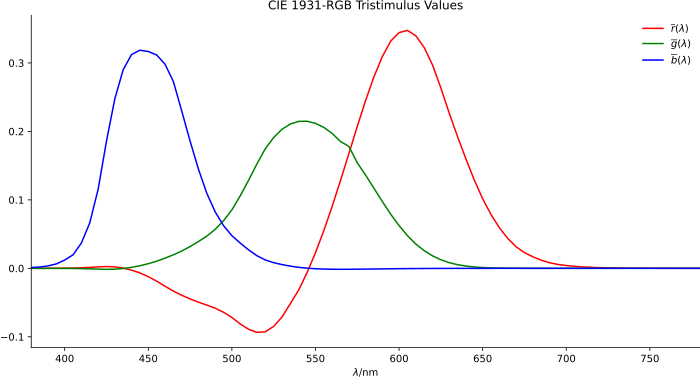
\includegraphics[width=0.8\textwidth]{./imgs/sec1/rgb-1931.pdf}
    \caption{CIE 1931-RGB色彩空间色彩匹配函数}
    \label{fig:tri-rgb}
 \end{figure}

从上文我们得知了RGB三基色,CIE在提出RGB系统的同时,通过实验确定确定了各个单波长的三刺激值,得到了色彩匹配函数(Color matching function,CMF),如图\ref{fig:tri-rgb}所示。色彩匹配函数是视觉系统的固有属性,是一个客观存在的量。我们只需将光谱数据与色彩匹配函数做一个积分、求和\eqref{eq:tri-rgb},便可以获取其RGB相关信息。通过对RGB进行归一化\eqref{eq:tri-rgb-n},便可以获取到色品坐标$(r,g)$,就能唯一确定一种颜色。

\begin{equation}
    \begin{aligned}
        R & =\int \overline{r}(\lambda)\cdot\psi(\lambda)\text{d}\lambda \quad\text{or}\quad R = \sum_{380\text{nm}}^{780\text{nm}} \overline{r}(\lambda)\cdot\psi(\lambda)\\
        G & =\int \overline{g}(\lambda)\cdot\psi(\lambda)\text{d}\lambda \quad\text{or}\quad G = \sum_{380\text{nm}}^{780\text{nm}} \overline{g}(\lambda)\cdot\psi(\lambda)\\
        B & =\int \overline{b}(\lambda)\cdot\psi(\lambda)\text{d}\lambda \quad\text{or}\quad B = \sum_{380\text{nm}}^{780\text{nm}} \overline{b}(\lambda)\cdot\psi(\lambda)\\
    \end{aligned}
    \label{eq:tri-rgb}
\end{equation}

\begin{equation}
    \begin{aligned}
        r & =\frac{R}{R+G+B}\\
        g & =\frac{G}{R+G+B}\\
        b & =\frac{B}{R+G+B} = 1-r-g\\
    \end{aligned}
    \label{eq:tri-rgb-n}
\end{equation}

但是从图\ref{fig:tri-rgb}中可以看出CIE 1931-RGB色彩空间色彩匹配函数中$r$存在负值,不方便计算以及不符合人类的直观感受,并且由于负值的存在,从$C=R+G+B$的三刺激值中无法直观地理解。为了消除这部分负值的影响以及均匀度的问题,CIE组织提出了几种由RGB空间线性、非线性变换得来的色彩空间,如XYZ、Lab、Luv。本文基于的题目便是当中的一种线性变换色彩空间--XYZ。

\subsection{XYZ色彩空间}

\begin{figure}[htbp]
    \centering
    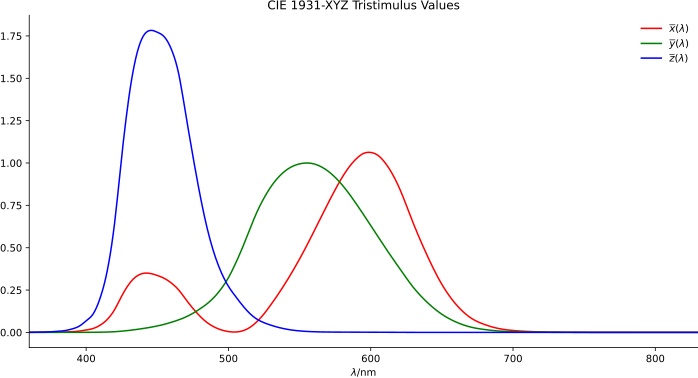
\includegraphics[width=0.8\textwidth]{./imgs/sec1/xyz-1931.pdf}
    \caption{CIE 1931-XYZ色彩空间色彩匹配函数}
    \label{fig:tri-xyz}
 \end{figure}

在CIE 1931-XYZ色彩空间空间中,虚构了X(红)、Y(绿)、Z(蓝)三原色,同时解决了亮度叠加($C=X+Y+Z$)与色彩匹配函数负值问题,色彩匹配函数如图\ref{fig:tri-xyz}所示。与RGB色彩空间一样,我们只需将光谱数据与色彩匹配函数做一个积分、求和\eqref{eq:tri-xyz},便可以获取其XYZ相关信息,其中$Y$为色光的亮度,$k$根据亮度$Y$的需求决定。通过对XYZ进行归一化\eqref{eq:tri-xyz-n},便可以获取到色品坐标$(x,y)$,也能唯一确定一种颜色。XYZ色彩空间三刺激值与RGB色彩空间三刺激值的线性转换如公式\eqref{eq:tri-xyz-rgb}所示。

\begin{equation}
    \begin{aligned}
        X & =k\int \overline{x}(\lambda)\cdot\psi(\lambda)\text{d}\lambda \quad\text{or}\quad R = k\sum_{380\text{nm}}^{780\text{nm}} \overline{x}(\lambda)\cdot\psi(\lambda)\\
        Y & =k\int \overline{y}(\lambda)\cdot\psi(\lambda)\text{d}\lambda \quad\text{or}\quad G = k\sum_{380\text{nm}}^{780\text{nm}} \overline{y}(\lambda)\cdot\psi(\lambda)\\
        Z & =k\int \overline{z}(\lambda)\cdot\psi(\lambda)\text{d}\lambda \quad\text{or}\quad B = k\sum_{380\text{nm}}^{780\text{nm}} \overline{z}(\lambda)\cdot\psi(\lambda)\\
        k & = \frac{1}{Y} (\frac{100}{Y},\frac{683}{Y})\\
    \end{aligned}
    \label{eq:tri-xyz}
\end{equation}

\begin{equation}
    \begin{aligned}
        x & =\frac{X}{X+Y+X}\\
        y & =\frac{Y}{X+Y+X}\\
        z & =\frac{Z}{X+Y+X} = 1-x-y\\
    \end{aligned}
    \label{eq:tri-xyz-n}
\end{equation}

\begin{equation}
    \begin{bmatrix}
        \overline{r}\\
        \overline{g}\\
        \overline{b}\\
    \end{bmatrix} = \begin{bmatrix}
    0.41846 & -0.15860 & -0.08283\\
    -0.09117 & 0.25243 & 0.01571\\
    0.00092 & -0.00255 & 0.17860\\
    \end{bmatrix}\begin{bmatrix}
        \overline{x}\\
        \overline{y}\\
        \overline{z}\\
    \end{bmatrix}
    \label{eq:tri-xyz-rgb}
\end{equation}


从上一小节我们曾提到,XYZ是RGB经转化而来的,由于本人的仿真所在的操作系统的是Windows,缺省的色彩模式为Standard RGB(sRGB),因此我们将此处的RGB默认为sRGB,XYZ转sRGB还需要一段非线性函数进行校正(gamma校正),sRGB转XYZ(Y=1)如公式\eqref{eq:trans-srgb2xyz}所示,XYZ(Y=1)转sRGB如公式\eqref{eq:trans-xyz2srgb}所示。

\begin{equation}
    \begin{aligned}
        \begin{bmatrix}
            sR^\prime\\
            sG^\prime\\
            sB^\prime\\
        \end{bmatrix} & = V^\prime = \left\{ \begin{matrix}
            \frac{V}{12.92} & V\leq 0.04045 \\
            (\frac{V+0.055}{1.055})^{2.4} & V> 0.04045 \\
        \end{matrix} \right.
        \\
        \begin{bmatrix}
            X\\
            Y\\
            Z\\
        \end{bmatrix} &= 
        \begin{bmatrix}
            0.4124 & 0.3576 & 0.1805\\
            0.2126 & 0.7152 & 0.0722\\
            0.0193 & 0.1192 & 0.9505\\
        \end{bmatrix}\begin{bmatrix}
            sR^\prime\
            sG^\prime\
            sB^\prime\
        \end{bmatrix} 
    \end{aligned}
    \label{eq:trans-srgb2xyz}
\end{equation}

\begin{equation}
    \begin{aligned}
        C_\text{linear} = \begin{bmatrix}
            R^\prime\\
            G^\prime\\
            B^\prime\\
        \end{bmatrix} &= 
        \begin{bmatrix}
            3.24062548& -1.53720797 & -0.49862860\\
            -0.96893071& 1.87575606 & 0.04151752\\
            0.05571012& -0.20402105 & 1.05699594\\
        \end{bmatrix}\begin{bmatrix}
            X\\
            Y\\
            Z\\
        \end{bmatrix} \\
        \begin{bmatrix}
            R\\
            G\\
            B\\
        \end{bmatrix} &= \left\{ \begin{matrix}
            \max(12.92\cdot C_\text{linear},0) & C_\text{linear}\leq 0.0031308 \\
            1.055(C_\text{linear}^\frac{1}{2.4}) - 0.055 & C_\text{linear}> 0.0031308 \\
        \end{matrix} \right.
    \end{aligned}
    \label{eq:trans-xyz2srgb}
\end{equation}

从公式中我们可以知道,理论上存在颜色相同而光谱不同的非纯色光,混色的方法有很多种。

CIE 1931-XYZ的色彩也是基于人测定的,由于一些较纯的色彩在实际中并不会用到以及新的实验,CIE提出了CIE 2006-XYZ色彩空间,其对xyz三刺激值做了一些修正(主要为蓝色),如图\ref{fig:tri-xyz-2}所示。从图中我们可以知道,除蓝色的峰值外,CIE 2006-XYZ色彩相较于CIE 1931-XYZ区别不大。

\begin{figure}[htbp]
    \centering
    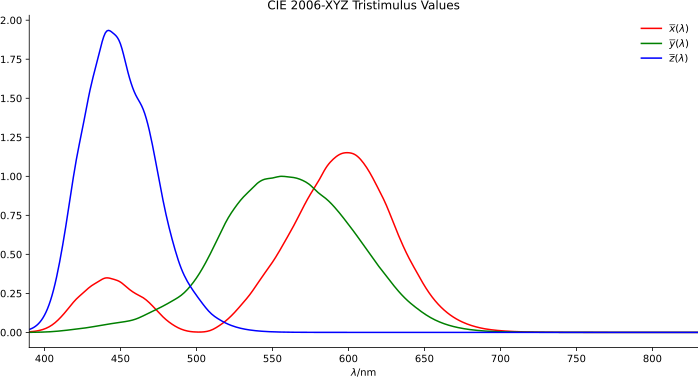
\includegraphics[width=0.8\textwidth]{./imgs/sec1/xyz-2006.pdf}
    \caption{CIE 2006-XYZ色彩空间色彩匹配函数}
    \label{fig:tri-xyz-2}
 \end{figure}